本研究の目的は, 配信に途中参加したユーザがダイジェスト視聴可能なP2Pライブストリーミングシステムを提案することである. この目的を達成するために2つの段階を考える. 1つ目の段階として, まずP2Pネットワーク内でダイジェストを生成することを考える. 動画コンテンツであったり, ライブ映像であっても, ダイジェストを生成するための専用の計算機やサーバを用意することが出来れば, 既存のダイジェスト生成方式を使える. しかし, 本研究ではP2Pライブストリーミングにおいてダイジェストを生成することを考えるため既存の手法は使えない. そこで, P2Pライブストリーミングに特化したダイジェスト生成方式を提案する. 2つ目の段階として, P2Pネットワーク内で作成したダイジェストを保持し, 広めるためのトポロジ設計を行うことである. システムはP2Pなのでダイジェストを管理する特別なサーバを用意することが出来ない. よって作成したダイジェストはサーバではなく各ピアが管理するため, 各ピアが役割を持ったトポロジを設計する.

%% 本研究の要求条件の1つは遅延や離脱耐性を考慮した階層型クラスタにすることである. もう1つの要求条件はネットワーク内のダイジェストを枯渇させないことである. 要求条件を達成するためにクラスタ内部の論理ホップ数は少なくなるように配置する. またダイジェストはクラスタ内ですべての種類が揃っているようにする. こうすることでダイジェストを取得するまでの論理ホップ数を軽減させることが出来る.

まず最初にダイジェスト生成方式についての提案方式を述べ, 次にトポロジ設計についての提案方式を述べる.
\section{ダイジェスト生成方式}
P2Pライブストリーミングを行う際に, 特別なサーバに頼ること無く参加している各ピアがダイジェストを生成出来るような方式を提案する. 本研究では3つの異なる手法に基づいたダイジェスト生成方式を提案する. 1つ目は「閾値に基づくダイジェスト生成方式」, 2つ目は「前後比較に基づくダイジェスト生成方式」, 3つ目は「最小二乗法に基づくダイジェスト生成方式」である.

本研究ではある特定の種類, 例えばスポーツなどの映像に特化したダイジェスト生成方式ではなく, どのような種類の映像にも適応可能な汎用的なダイジェスト生成方式を目指す. そのため, 私はP2Pライブストリーミングシステムに参加しているユーザ数に着目した. ユーザ数は1つのコンテンツを視聴しているユーザの数を意味する. ユーザ数はどの種類の映像のコンテンツであっても共通の指標として利用できるため, 汎用的なダイジェスト生成方式を目指す私のシステムに適している. ユーザ数はコンテンツの継続時間によって増減し, 特定の時刻のユーザ数が多いほど注目度が高いことを意味する. その注目度の高い特定の時刻のコンテンツの内容をダイジェストとして利用することを考える. 継続時間によって変化するユーザ数を用いて, ユーザ数増減グラフ\ref{fig:zogen}を作成することが出来る. 提案する3つの方式では, ユーザ数増減グラフにおいて突出している部分「突出点」を発見することによりダイジェストを作成する.

\begin{figure}[h]
  \centering
  \includegraphics[width=1\hsize]{fig/zogen.eps}
  \caption{あるコンテンツのユーザ数増減グラフ}
  \label{fig:zogen}
\end{figure}

ダイジェスト生成方式を提案するにあたり, 達成すべき要求条件を以下にあげる.

\begin{itemize}
\item 特定の種類のコンテンツに依存しないダイジェスト生成方式であること
\item ライブストリーミングに特化したダイジェスト生成方式であること
\item 生成されたダイジェストの映像によってコンテンツの内容の全体把握が出来ること
\end{itemize}

\subsection{閾値に基づくダイジェスト生成方式}
1つ目は「閾値に基づくダイジェスト生成方式」である. これはユーザ数が増加している時を始点, ユーザ数が減少している時を終点とし, 始点から終点までで最もユーザ数の多い点を「突出点」として抽出する方式である. ユーザ数の増加率と減少率をそれぞれ閾値として決定し, それぞれの値を超えた時を始点または終点として定義する. これは以下の式\ref{siki:sikiiti}に従う.

\begin{eqnarray}
\frac{X_{t+T}-X_{t}}{X_{t}} \geq ThならばX_{t}は始点 \nonumber \\
(X_{t}は時刻tにおけるユーザ数,Tは一定期間, Thは閾値)&&
\label{siki:sikiiti}
\end{eqnarray}

図\ref{fig:sikiiti}は閾値に基づくダイジェスト生成方式を適応したグラフである. 縦に赤い線が始点であり, 縦に青い線が終点である. 始点は数分間のユーザ数の増加率を計算したのち, その増加率が閾値を超えた点を示している. 終点は数分間のユーザ数の減少率を計算したのち, その減少率が閾値を超えた点を示している. 縦に緑の線は「突出点」を示しており, この部分をダイジェストとして抽出する.

\begin{figure}[h]
  \centering
  \includegraphics[width=1\hsize]{fig/sikiiti.eps}
  \caption{閾値に基づくダイジェスト生成方式を適応したグラフ}
  \label{fig:sikiiti}
\end{figure}

\subsection{前後比較に基づくダイジェスト生成方式}
2つ目は「前後比較に基づくダイジェスト生成方式」である. これは, ある点についてユーザ数が前後で増加かつ減少している場合を「突出点」として抽出する方式である. この方式も1つ目の方式と同様にユーザ数の増加率と減少率をそれぞれ閾値として決定し, それぞれの値を超えた場合に「突出点」を決定する. これは以下の式\ref{siki:zengo}に従う.

\begin{eqnarray}
\frac{X_{t}-X_{t-T}}{X_{t}}>ThZokaかつ\frac{X_{t+T}-X_{t}}{X_{t}}>ThGenならばX_{t}がダイジェスト \nonumber \\
(X_{t}は時刻tにおけるユーザ数, Tは一定期間, ThZokaとThGenは閾値) &&
\label{siki:zengo}
\end{eqnarray}

図\ref{fig:zengo}は前後比較に基づくダイジェスト生成方式を適応したグラフである. 縦に緑の線は「突出点」を示しており, この部分をダイジェストとして抽出する. 1つ目の方式との違いは, 先に「突出点」となる候補を探し, その点が正しい「突出点」であるかを前後の増減率を計算して決定している点である.

\newpage

\begin{figure}[h]
  \centering
  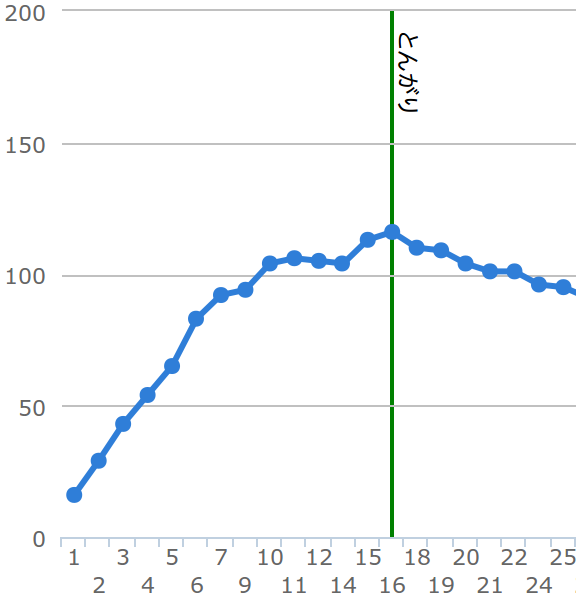
\includegraphics[width=1\hsize]{fig/zengo.eps}
  \caption{前後比較に基づくダイジェスト生成方式を適応したグラフ}
  \label{fig:zengo}
\end{figure}

\subsection{最小二乗法に基づくダイジェスト生成方式}
3つ目は「最小二乗法に基づくダイジェスト生成方式」である. これは, ユーザ数増減グラフに最小二乗法を適応し直線の重なりが鋭角な点を「突出点」とし抽出する方式である. 最小二乗法を適応した際の直線の重なりの角度を閾値として決定し, その値を超えた場合にその点を「突出点」として決定する. これは以下の式\ref{siki:jijo}に従う.

\begin{eqnarray}
\arctan \left(\frac{line2\_slope - line1\_slope}{1+line2\_slope*line1\_slope}\right) < ThAngle \nonumber \\
ならば直線の重なり部分がダイジェスト \nonumber \\
(line1\_slopeおよびline2\_slopeは直線の傾き, ThAngleは閾値) &&
\label{siki:jijo}
\end{eqnarray}

図\ref{fig:jijo}は最小二乗法に基づくダイジェスト生成方式を適応したグラフである. 点と点の間のカラフルな線が最小二乗法を適応した時の直線であり, 縦に緑の線が「突出点」を示しており, この部分をダイジェストとして抽出する.

\begin{figure}[h]
  \centering
  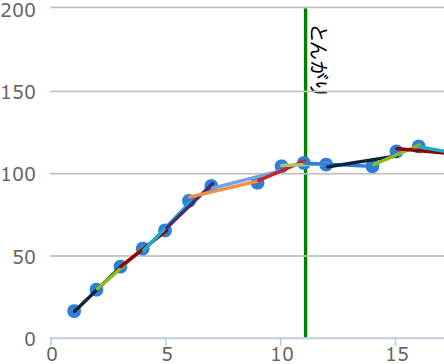
\includegraphics[width=1\hsize]{fig/jijo.eps}
  \caption{最小二乗法に基づくダイジェスト生成方式を適応したグラフ}
  \label{fig:jijo}
\end{figure}

\subsection{既存のダイジェスト生成方式との比較}
関連研究であげた既存のダイジェスト生成方式との比較の結果を以下に示す. 橋本らの提案したスポーツ映像を対象とした方式を「方式1」, 熊野らの提案した野球の実況中継映像を対象とした方式を「方式2」, 本研究で提案する方式を「提案方式」とする.

\begin{table}[h]
  \caption{実行環境}
  \label{tbl:EvalEnv}
  \centering
      {\small
        \begin{tabular}{|l|l|l|l|}
          \hline
          & 方式1 & 方式2 & 提案方式 \\ \hline \hline
          リアルタイム性 & × & ○ & ○ \\ \hline
          P2Pへの対応 & × & × & ○ \\ \hline
          汎用性 & × & × & ○ \\ \hline
        \end{tabular}
      }
\end{table}

方式1や方式2に比べ, 提案方式ではP2Pライブストリーミングにおいて汎用的なダイジェスト生成方式であることがわかる.

\section{トポロジ設計}
これまでは, P2Pライブストリーミングにおいて汎用的なダイジェスト生成方式について述べてきた. ここでは生成されたダイジェストをP2Pネットワーク内で保持し, それを拡散させるためのトポロジ設計を提案する.

トポロジの構成としては主にツリー構造とメッシュ構造が存在する. ツリー構造とは, 1つのノードが複数の子を持ち, 1つの子が複数の孫を持つという形になっており, 枝分かれをしながら階層が深くなっていく構造のことである. 木が幹から枝に, 枝から葉に分かれていく様子に似ていることからツリー構造と言われている. ツリー構造は構造が単純なため構築が容易であるが, その反面1つのノードが居なくなるとそれより下の子全員が切り離されてしまうので耐故障性に弱いという特徴がある. メッシュ構造とはツリー構造のように親と子のみと接続するのではなく, 複数のノードが接続し相互に通信を行う構造のことである. 複数のノードが接続しているので網の目(mesh)のように見えるためメッシュ構造と言われている. メッシュ構造はツリー構造のように特定のノードからのみ受信するのではなく, 複数のノードから受信できるので耐故障性に優れている. しかし必然的に各ノードの接続数が増えるため, 遅延が大きくなってしまうという問題がある. これらの問題を解決する構造として, 関連研究で紹介した複数クラスタ型が登場した. 複数クラスタ型はツリー構造のように中継ノードにストリームを渡し, 各中継ノードはそれぞれクラスタを作成してクラスタの中ではメッシュ構造のように複数のノード同士が接続している構造である. 複数クラスタはツリー構造とメッシュ構造の欠点を補っている. 本研究では複数クラスタ型のトポロジ設計にする.

複数クラスタ型では中継ノードを選ぶ必要がある. また, 本研究ではP2Pのライブストリーミングシステムを対象としているため, ダイジェストを管理するためのサーバを用意することが出来ない. そのため, 生成されたダイジェストは特定のノードに管理させることにする. さらに, 中継ノードへの負担を軽減するためにクラスタ内へストリームを広めるためのノードも必要である. このように, 各ノードに役割を持たせたトポロジ設計にする. 中継ノードを「ゲートノード」, ダイジェストを管理をするノードを「ダイジェストノード」, クラスタ内へストリームを広めるためのノードを「セミゲートノード」と定義する.

トポロジ設計を提案するにあたり, 達成すべき要求条件を以下にあげる.

\begin{itemize}
\item ライブストリーミングの映像を見れること
\item ダイジェストを視聴できること
\item
\end{itemize}

%% ここから下ちゃんと書く

\subsection{配信内容に対するコメント}

本研究で提案するP2Pライブストリーミングシステムでは, 参加ユーザが配信内容に対して自由にコメント投稿が出来ることを想定する. コメントは1ユーザにつき何回でも投稿出来るものとする. 各ユーザが投稿したコメント数はシステム内で管理し, 各ノードの役割を決定するために指標として利用する.

\subsection{ノードの役割}
各ノードにはそれぞれ役割を割り当てる.

\subsubsection{ゲートノード}
配信者ノードから配信されたコンテンツのパケットをクラスタ内で一番最初に取得する. また, 他のクラスタのゲートノードと繋ぎコンテンツのパケットを送受信する役割を担う.

\subsubsection{セミゲートノード}
クラスタ内でゲートノードから受信したパケットをクラスタ内部に拡散する役割を担う.

\subsubsection{ダイジェストノード}
ダイジェストを保有し, 新規参加ノードへ送信する役割を担う.

\subsubsection{その他のノード}
その他にトラッカーサーバが存在する. トラッカーサーバは各ノードのコメント数, 帯域幅, ホップ数等を計算しする. 全てのノードが繋ぎ, 全てのノードの情報を管理する. また, どの役割にも属さないものをノーマルノードとする.

\subsection{ノードの役割決定方法}
ノードの役割を決定する方法について述べる. 図\ref{fig:role}に図解したものを載せる.

\begin{figure}[h]
  \centering
  \includegraphics[width=1\hsize]{fig/role.eps}
  \caption{ノードの役割を決定する方法}
  \label{fig:role}
\end{figure}


\subsection{ノード間接続方法}
図\ref{fig:topology}は提案システムのトポロジの様子である. 2つのクラスタがあり, その外側の接続と, クラスタ内の接続について示している.

まず, クラスタ外部での接続方法を示す. 配信者ノードは全てのゲートノードと接続する. 1つのゲートノードは他のクラスタのゲートノード1つずつと接続することとする.

次にクラスタ内部での接続方法を示す. 1つのゲートノードは他の全てのゲートノードと接続する. また対応するセミゲートノード1つずつと接続する. 1つのセミゲートノードはダイジェストノードの3分の1と接続する. またノーマルノード2つずつと接続する. 1つのダイジェストノードはダイジェスト未取得ノーマルノード全てと接続する. ノーマルノードはノーマルノードの4分の1と接続することとする.

\begin{figure}[h]
  \centering
  \includegraphics[width=1\hsize]{fig/topology.eps}
  \caption{提案システムのトポロジ}
  \label{fig:topology}
\end{figure}

\subsection{新規参加ピアについて}
新規参加ピアの行動について述べる. 新規参加ピアはネットワーク接続時に配信者ノードにつなぐ. その後, トラッカーサーバが新規参加ピアの帯域や各クラスタへの論理ホップ数を計算し, 最も論理ホップ数の小さいクラスタに配置される(もしくはRTTの小さいクラスタに配置される). クラスタに配置された後, ダイジェスト保有ピアからダイジェストを受け取り, ダイジェストの映像を見ることが出来る.

新規参加ピアの行動のシーケンス図

\subsection{再構築のタイミング}
再構築のタイミングは3つある. 1つ目は新規参加ピアがダイジェストを取得し終わった時である. ダイジェスト保有ノードと接続を切断したあと, 帯域に応じて接続数を決定する. 帯域が十分に高い場合にはセミゲートノードになる. 2つ目はコメント数が一定数を超えた時である. この場合, 対象のノードはダイジェスト保有ノードになる. 3つ目はノードが離脱した時である. 離脱ノードに接続していたピアは帯域に応じた接続数を維持するように他のピアと接続する. 特にゲートノードが離脱した場合はセミゲートノードが即座にゲートノードになる. また, 特にセミゲートノードが離脱した場合はクラスタの中で帯域が高いピアがセミゲートノードになる.

\subsection{既存のトポロジ設計との比較}
関連研究であげた既存のトポロジ設計との比較の結果を以下に示す. 比較する全てのトポロジは複数クラスタ型である. Yang Guoの提案したHCPSを「HCPS」, 元橋らの提案した重畳クラスタ木方式の動画配信システムを「重畳型」, Huey-Ing Liuらの提案したMeTreeを「MeTree」, 本研究で提案する方式を「提案方式」とする.

\begin{table}[h]
  \caption{実行環境}
  \label{tbl:EvalEnv}
  \centering
      {\small
        \begin{tabular}{|c|c|c|c|c|} \hline
          & HCPS & 重畳 & MeTree & 提案 \\ \hline \hline
          \shortstack{ダイジェ \\ スト} & なし & なし & なし & あり\\ \hline
          クラスタ & \shortstack{完全 \\ 結合} & \shortstack{一部 \\ メッシュ} & \shortstack{一部 \\ メッシュ}  & \shortstack{一部 \\ メッシュ}\\
          \hline
          \shortstack{ゲート \\ ノード} & \shortstack{高帯域 \\ ピア} & \shortstack{滞在時間 \\ の長い \\ ピア} & \shortstack{高帯域 \\ ピア} & \shortstack{高帯域+ \\ コメント \\ 量の多い \\ ピア} \\
          \hline
        \end{tabular}
      }
\end{table}

